\documentclass[10pt]{scrartcl}

\usepackage[utf8]{inputenc}
\usepackage{tabularx}
\usepackage{longtable}
\usepackage[ngerman]{babel}
\usepackage[automark]{scrpage2}
\usepackage{amsmath,amssymb,amstext}
%\usepackage{mathtools}
\usepackage[]{color}
\usepackage[]{enumerate}
\usepackage{graphicx}
\usepackage{lastpage}
\usepackage[perpage,para,symbol*]{footmisc}
\usepackage{listings} 
\usepackage[pdfborder={0 0 0},colorlinks=false]{hyperref}
\usepackage[numbers,square]{natbib}
\usepackage{color}
\usepackage{colortbl}
\usepackage[absolute]{textpos}
\usepackage{float}
%\usepackage[colorinlistoftodos,textsize=small,textwidth=2cm,shadow,bordercolor=black,backgroundcolor={red!100!green!33},linecolor=black]{todonotes}

\lstset{numbers=left, numberstyle=\tiny, numbersep=5pt, breaklines=true, showstringspaces=false} 
\restylefloat{figure}

%changehere
\def\titletext{Bericht TT2P 1}
\def\titletextshort{Praktikum 1}
\author{Steffen Brauer, André Harms,\\ Florian Johannßen, Jan Meier,\\ Florian Ocker, Olaf Potratz,\\ Torben Woggan}

\title{\titletext}

%changehere Datum der Übung
\date{10.06.2012}

\pagestyle{scrheadings}
%changehere
\ihead{TT2, Neitzke}
\ifoot{Generiert am:\\ \today}

\cfoot{Steffen Brauer, André Harms,\\ Florian Johannßen, Jan Meier,\\ Florian Ocker, Olaf Potratz,\\ Torben Woggan}


\ohead[]{\titletextshort}
\ofoot[]{{\thepage} / \pageref{LastPage}}

\setlength{\parindent}{0.0in}
\setlength{\parskip}{0.1in}

\begin{document}
\maketitle

\setcounter{tocdepth}{3}
\tableofcontents

%	\listoftables                                 												% 
	\listoffigures  
%	\lstlistoflistings	
\newpage
\section{Grundlagen}
Verstärkendes Lernen oder Bestärkendes Lernen (engl. Reinforcement Learning), ist der Überbegriff für eine Reihe von Methoden zum Maschinellen Lernen (engl. Machine Learning). Beim Verstärkenden Lernen gibt es keine Vorgabe von Trainingsbeispielen, der Agent kann nur aus den eigenen Erfahrungen lernen. Ein Agent befindet sich immer in einer Umwelt, über die er Informationen besitzen muss. Ein real existierender Agent (im Gegensatz zu einem Agenten, der nur in einer Simulation virtuell vorhanden ist) nimmt Informationen über die Umwelt mit Sensoren wahr. Auf die Informationen kann er mit Aktionen reagieren, z.B. ein mechanisches Teil bewegen. Das Handeln des Agenten besteht somit aus einer Folge von Aktionen. Das Ziel des Verstärkenden Lernens ist nun, dass der Agent selbständig erkennen kann, welche Aktion die günstigste ist. Dies muss er lernen können. Dieser Lernprozess basiert auf positiven Belohnungen und negativen Belohnungen (Kosten). Höhere Belohnungen werden vom Agenten bevorzugt. Der Agent lernt, wie die Aktionen belohnt werden, somit kann er in Zukunft bessere Entscheidungen treffen (Verstärkung). Die Verstärkung kann auch erst zu spät einsetzen (z.B. nach Ende eines Spiels), so dass das gelernte Wissen erst später eine Rolle spielt (z.B. beim nächsten Spiel).

Konkret wird vom Zeitpunkt $t$, dem Zustand $s_t$, der Aktion $a_t$ und der Belohnung (Reward) $r_t$ zum Zeitpunkt $t$ gesprochen. Der Agent wählt zum Zeitpunkt $t$ eine Aktion $a_t$ und gelangt dadurch von Zustand $s_t$ in Zustand $s_{t+1}$ und erhält daraufhin eine Belohnung $r_{t+1}$. Im Zustand $s_{t+1}$ wählt er nun wiederum eine Aktion $a_{t+1}$.

Die Belohnungen und der Folgezustand werden dabei als Teil des Modells der Umgebung angesehen. Allerdings ist die Umgebung im Allgemeinen nicht-deterministisch. Das Ausführen einer bestimmten Aktion in einem bestimmten Zustand muss somit nicht immer im gleichen Folgezustand resultieren. Der Übergang in die Folgezustände basiert aber immer auf den gleichen Wahrscheinlichkeiten, die sich im Laufe der Zeit auch nicht verändern, man sagt die Umgebung ist stationär.

\section{Dynamische Programmierung}

Dynamische Programmierung ist eine Methode zum algorithmischen Lösen von Optimierungsproblemen und kann als Spezialfall von Reinforcement Learning angesehen werden. Dynamische Programmierung kann erfolgreich eingesetzt werden, wenn das Problem aus mehreren gleichartigen Teilproblemen besteht. Dabei muss sich eine optimale Lösung des Problems aus optimalen Lösungen der Teilprobleme zusammensetzen. Zuerst werden die optimalen Lösungen der kleinsten Teilprobleme berechnet. Diese werden dann geeignet zu einer Lösung eines nächstgrößeren Teilproblems zusammenzusetzen. Diese Schritte werden wiederholt. Einmal berechnete Teilergebnisse werden gespeichert, um bei nachfolgenden Berechnungen gleichartiger Teilprobleme auf diese Zwischenlösungen zurück greifen zu können, anstatt eine neue Berechnung anstellen zu müssen. 

Die Voraussetzung, um dynamische Programmierung anwenden zu können ist ein vollständiges Modell. Dies bedeutet, dass alle Zustände inklusive ihrer Belohnungen und Folgezustände in Abhängigkeit von Ausgangszustand und einer Aktion bekannt sind.
Somit sind $\mathcal{P}^{a}_{ss'}$ und $\mathcal{R}^{a}_{ss'}$ bekannt und müssen nicht erst durch Erfahrungen geschätzt werden.

\subsection{Policy Evaluation}
Policy Evaluation beschreibt die Berechnung von Zustandswerten bezüglich einer gegebenen Strategie (Policy) entsprechend der Bellman-Gleichung. Es werden für eine gegebene Strategie $\pi$ die zugehörigen Wertefunktionen $V^{\pi}$ berechnet. Dabei werden episodische Probleme betrachtet, so dass ein künstlicher Endzustand $S_{final}$  und ein erweiterter Zustandsraum $S^+=S\cup{S_{final}}$ ($S$ mit $S_{final}$) definiert werden kann. Das Ergebnis wird iterativ ermittelt (bzw. approximiert). Hierzu wird eine aufeinander aufbauende Wertereihenfolge $V_0, V_1 ... V_n$ für alle Zustände in $s \in S$ generiert. $V_0$ kann dabei beliebig für alle Zustände beliebig gewählt werden. Durch Iteration der Bellman-Gleichung erfolgt eine Näherung an die Wertfunktionen der Zustände:

\begin{align*}
V^\pi_{k+1}(s) = \sum\limits_{a} \pi(s,a) \sum\limits_{s'}\mathcal{P}^a_{ss'}[\mathcal{R}^a_{ss'}+\gamma V^\pi_k(s')]
\end{align*}

Dies geschieht für alle Zustände in $S^+$. Vor der Iteration wird $V^\pi_k$  (beim Start ist $k=0$) mit Null initialisiert. Die Iteration erfolgt von $k=0$ bis unendlich, jedoch wird abgebrochen sobald die  Abbruchbedingung erfüllt ist. Durch ausreichend langes Iterieren tastet man sich beliebig nahe an die echte Wertfunktion heran. Als Abbruchbedigung dient folgender Term:

\begin{align*}
\max\limits_{s\in S^+} |V_{k+1}(s)-V_k(s)|
\end{align*}

Es wird hierbei der größte Differenz-Wert zwischen zwei Schritten genommen und  auf Überschreiten des Schwellwertes überprüft.\\
In der Abbildung \ref{fig:policyevaluation} ist der Pseudocode des Algorithmus aufgeführt.

\begin{figure}[htc]
    \centering
    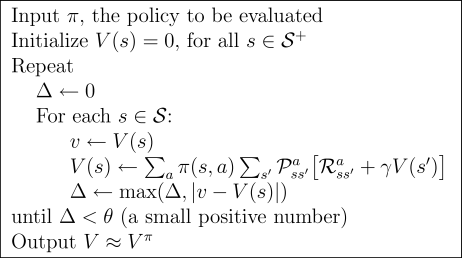
\includegraphics[width=0.7\textwidth]{Grafiken/21pe.png}
    \caption{Pseudocode des Policy-Evaluation Algorithmus}
    \label{fig:policyevaluation}
\end{figure}

\subsection{Policy Improvement}
Grund für das Ermitteln einer Wertfunktion, ist das Bestreben eine bessere Strategie zu finden. Wenn $V^\pi$ eine beliebige Wertfunktion für die  Strategie $\pi$ ist,  ist es interessant, ob für einen Zustand $s$ eine andere Aktion $a\neq\pi(s)$   gewählt werden soll, oder aber die alte Aktion $a=\pi(s)$ beibehalten werden soll.
Es gibt verschiedene Möglichkeiten, diese  Entscheidung zu treffen. Eine ist, eine beliebige Aktion $a$ zu wählen und dann mit der bestehenden Strategie $\pi$ fortzufahren. Der Wert durch Ausführen dieses $a$s ist durch $Q^\pi(s,a)$ beschrieben. Die Frage, die sich stellt, ist: Ist $Q^\pi(s,a)$ besser als $V^\pi(s)$?
Ist dies der Fall, sollte die ermittelte Aktion $a$ der bestehenden Strategie vorgezogen werden.

Seien $\pi$ und $\pi'$ ein beliebiges Paar von Strategien, so dass für alle $s \in S$ gilt:
\begin{align*}
Q^\pi(s,\pi'(s)) \ge V^\pi(s)
\end{align*}

Dann ist Strategie $\pi'$  mindestens so gut wie $\pi$, was wiederum bedeutet:

\begin{align*}
V^{\pi'}(s) \ge V^\pi(s)
\end{align*}

Mathematisch ausgedrückt kann die beste Aktion $a$ für den Zustand $s$ folgendermaßen gefunden werden:

\begin{align}\label{policy-improvement}
\pi'(s) &= arg\underset{a}{max}\sum_{s'}\mathcal{P}^a_{ss'}[\mathcal{R}^a_{ss'}+\gamma V^\pi(s')]
\end{align}

Die Funktion $argmax$ gibt gibt den Funktionsparameter zurück, für den die Funktion den höchsten Wert ergibt\footnote{Z.B. wenn $f(1)=10, f(2) = 50, f(3) = 25$ dann würde $arg\underset{x}{max}f(x)$ den Wert $2$ zurückliefern}. In Gleichung \ref{policy-improvement} wird somit das $a$ zurückgeben, was den höchsten Wert ergibt und so eine Strategie-Verbesserung erreicht. $\pi'$ stellt die verbesserte Strategie dar.

\subsection{Policy Iteration}
\subsection{Value Iteration}
Bei einer Strategie $\pi : S \rightarrow A $ werden Zustände auf Aktionen abgebildet. Die Strategie ist optimal, sofern sie Belohnung $r$ maximiert wird. Die abgeschwächte Belohnung einer Strategie $\pi$ kann durch folgende Gleichung berechnet werden:
\begin{align}\label{gleichungvp}
V^{\pi}(s_t) &= r_t + \gamma r_{t+1} + \gamma^2r_{t+2} + ... = \sum^{\infty}_{i=0} \gamma^ir_{t+1}
\end{align}
Die Variable $\gamma$ stellt eine Konstante dar dessen Wert zwischen null und eins angesiedelt ist: $0 \geq \gamma < 1$. Die Variable sorgt dafür, das ein weiter in der Zukunft liegendes Feedback abgeschwächt wird. Hierdurch wird die direkte Belohnung $r_t$ am stärksten gewichtet.

Eine Strategie ist optimal, sofern sie ebenso gut oder besser als anderen Strategien ist. 
Mathematisch kann dies folgendermaßen ausgedrückt werden, hierbei stellt $\pi^*$ die optimale Strategie dar:
\begin{align}\label{voptimal}
V^{\pi*}(s)\geq V^\pi(s)
\end{align}
Im Folgendem wird $V^{\pi*}$ mit $V^*$ bezeichnet.

Basierend auf dem Bellman-Prinzipg ist es möglich durch Optimierung einzelner Aktionen eine optimale Strategie zu finden. Gesucht ist eine optimale Strategie, die die Gleichungen \ref{gleichungvp} und \ref{voptimal} erfüllt. Somit kann folgende Gleichung aufgestellt werden:
\begin{align}
V^*(s_t) &= \underset{a_t,a_{t+1}, a_{t+2},...}{max}(r_t(s_t,a_t) + \gamma r_t(s_{t+1},a_{t+1}) + \gamma r_t(s_{t+2},a_{t+2}) + ...)
\end{align}
Da die direkte Belohnung $r(s_t, a_t)$ nicht von den Nachfolgezuständen und Belohnungen abhängt sondern nur  von $s_t$ und $a_t$ kann die Maximierung aufgeteilt werden. Wodurch sich folgende Gleichungen ergeben:
\begin{align}
V^*(s_t) &= \underset{a_t,a_{t+1}, a_{t+2},...}{max}[r(s_t, a_t) + \gamma \underset{a_{t+1},a_{t+2},...}{max}(r_t(s_{t+1},a_{t+1}) + \gamma r_t(s_{t+2},a_{t+2}) + ...)]\\
&= \underset{a_t}{max}[r(s_t, a_t)+\gamma V^*(s_{t+1})]\label{vmaximierung}
\end{align}
Die Gleichung \ref{vmaximierung} kann zu folgender Gleichung  vereichfacht werden:
\begin{align}\label{bellmangleichung}
V^*(s) &= max[r(s,a) + \gamma V^*(\delta(s,a))]
\end{align}
Diese Gleichung sagt aus, dass zur Berechnung von $V^*(s)$ die direkte Belohnung zu den mit dem Faktor $\gamma$ abgeschwächten Belohnungen aller Nachfolgezustände addiert wird. Sofern $V^*(\delta(s,a))$ bekannt ist ergibt sich $V^*(s)$ durch eine einfache lokale Optimierung über alle im Zustand $s$ möglichen Aktionen $a$. Hierdurch entspricht Gleichung \ref{bellmangleichung} dem Bellman-Prinzip und wird somit als Bellman-Gleichung bezeichnet.

Die optimale Strategie $\pi^*(s)$ führt im Zustand $s$ eine Aktion aus, die zum maximalen Wert $V^*$ führt. Somit gilt folgende Gleichung:
\begin{align}
\pi^*(s) = \underset{a}{argmax}[r(s,a) + \gamma V^*(\delta(s,a))]
\end{align}
Aus der Rekursionsgleichung \ref{bellmangleichung} ergibt sich folgende Iterationsvorschrift zur Berechnung von $V^*$:
\begin{align}
\widehat{V}(s) = \underset{a}{max}[r(s,a) + \gamma \widehat{V}(\delta(s,a))]
\end{align}
Dieses Verfahren zur Berechnung von $V^*$ wird als ``Value Iteration'' bezeichnet. 
Abbildung \ref{valueiteration} zeigt den Algorithmus in Form von Pseudocode.\\
Zu Beginn des Verfahrens wird $\widehat{V}$ für alle Zustände mit $0$ initialisiert. Darauffolgend wird für jeden $\widehat{V}(s)$ für jeden Zustand aktualisiert indem rekusriv auf den Wert $\widehat{V}(\delta(s,a))$ des besten Nachfolgezustands zugegriffen wird.

\begin{figure}[htc]
    \centering
    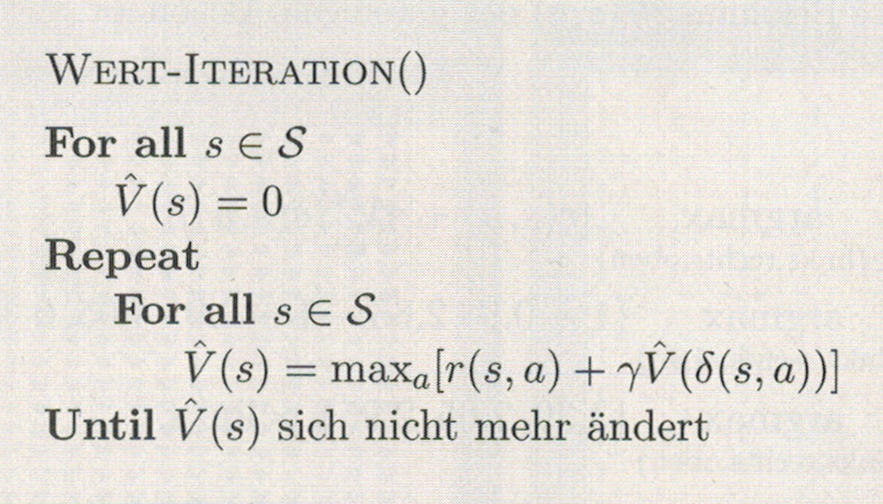
\includegraphics[width=0.6\textwidth]{Grafiken/value-iteration.png}
    \caption{Pseudocode des Value-Iteration Algorithmus}
    \label{valueiteration}
\end{figure}

\section{Temporal Difference Learning}

\section{Fazit}

\end{document}

